\subsection{Animieren der aktiven Trips}
\label{sub:animieren_der_aktiven_trips}
  Nachdem die Daten für alle aktiven Trips im Client ankommen, kann für jeden Trip ein Vehicle erstellt werden. In einem Animation-Loop wird für jedes Vehicle pro Frame, eine neue Position berechnet und die Karte wird mit der neuen Position aktualisiert. Der Algorithmus dafür ist in Pseudo-Code in Listing \ref{alg:animate_algorithmus} beschrieben.

  \begin{algorithm}[H]
    \caption{Animate Vehicle}\label{alg:animate_algorithmus}
    \begin{algorithmic}[1]
      \Procedure{animateVehicle}{}
        \State ServerQueryTimer $\gets$ 30 Seconds
        \State Vehicles $\gets$ Vehicles Inside Bounding Box
        \State Trips $\gets$ Requested Trips
        \Function{animate}{timestamp}
          \ForAll{Vehicles as Vehicle} \State{
            \If{Vehicle started its Trip} 
              \State \Call{calculateVehiclePosition}{Vehicle}
            \EndIf
            \If{Vehicle not started its Trip}
              \State \Call{checkVehicleActivity}{Vehicle, Trips}
            \EndIf
            \State \Call{checkIfVehicleHasFinished}{Vehicle}
            \State \Call{updateMapWithNewPositions}{Vehicles}
          }\EndFor

          \If{ServerQueryTimer Expired} 
            \State Query Server for New Trips
            \State ServerQueryTimer $\gets$ 30 Seconds
          \EndIf

          \State \Call {animate}{timestamp}
        \EndFunction
        
      \EndProcedure
    \end{algorithmic}
  \end{algorithm}

  Innerhalb dieses Animation-Loops passieren mehrere Dinge. Zuerst wird geprüft ob sich ein Vehicle überhaupt im Sichtbereich des Anwenders befindet. Trifft das zu, wird für eben diese Vehicle die Distanzen berechnet und die Position des Vehicles entlang der Polyline interpoliert. Falls das Vehicle seinen Trip noch nicht begonnen hat, wird überprüft ob das immer noch der Fall ist. Anschließend werden alle Vehicle geprüft, ob sie ihren Trip erledigt haben. Danach wird die Karte mit den neuen Positionen der Vehicle aktualisiert. Während all dies geschieht, läuft ein Timer mit, der nach dem Ablaufen von 30 Sekunden den Server nach neuen Trips abfrägt.

  Das Ergebnis ist die Animation aller Vehicle der momentan aktiven Trips (Abbildung \ref{fig:prozess/animate_all_vehicles}).

  \begin{figure}[htbp]
    \begin{center}
      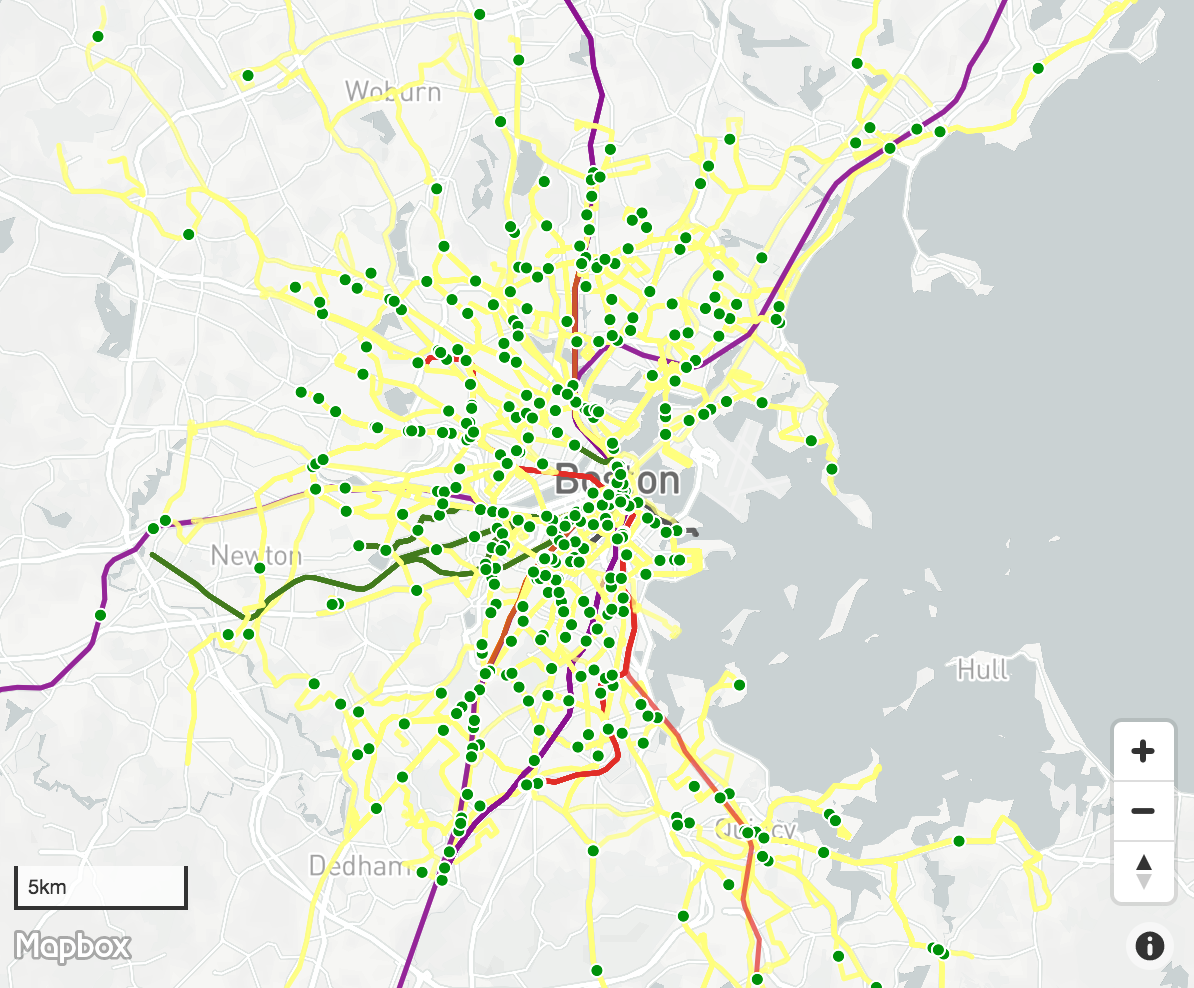
\includegraphics[width=0.7\textwidth]{prozess/animate_all_vehicles}
      \caption{Animieren aller Vehicles auf der Karte}
      \label{fig:prozess/animate_all_vehicles}
    \end{center}
  \end{figure}
  
  
  
% subsection animieren_der_aktiven_trips (end)